% INFORMS 2026 Data Mining Society Data Challenge — written report
% NOTE: all figures quoted here are regenerated by `python3 canonical.py` into
% CANONICAL.md. After the freeze rebuild, re-verify §6 against that file.
\documentclass[10pt,letterpaper,twocolumn]{article}
\usepackage[margin=0.72in]{geometry}
\usepackage{times}
\usepackage{amsmath,amssymb}
\usepackage{booktabs}
\usepackage{graphicx}
\usepackage[table]{xcolor}
\usepackage[colorlinks=true,linkcolor=black,citecolor=black,urlcolor=black]{hyperref}
\usepackage{titlesec}
\usepackage{caption}
\captionsetup{font=small,labelfont=bf,skip=3pt}
\titlespacing*{\section}{0pt}{6pt}{3pt}
\titlespacing*{\subsection}{0pt}{5pt}{2pt}
\titleformat{\section}{\normalfont\large\bfseries}{\thesection}{0.6em}{}
\titleformat{\subsection}{\normalfont\normalsize\bfseries}{\thesubsection}{0.6em}{}
\setlength{\abovedisplayskip}{4pt}
\setlength{\belowdisplayskip}{4pt}
\setlength{\parskip}{0pt}
\newcommand{\rmsev}[1]{\texttt{#1}}

\title{\vspace{-2.2em}\textbf{What Is Recoverable?}\\[2pt]
\large An Error-Budget Approach to County-Transfer\\Outage Forecasting}
\author{\normalsize INFORMS 2026 DMS Data Challenge}
\date{\vspace{-1em}}

\begin{document}
\maketitle
\vspace{-1.5em}

\begin{abstract}\small
\noindent We forecast hourly county Outage Severity Index (OSI) at four horizons
for 63 counties never seen in training, through a two-wave March 2026 wind event.
Rather than searching model space, we began by measuring \emph{how the
irreducible error decomposes}, because that determines which classes of
intervention can pay at all. The diagnosis --- made before the experiments, from
cached out-of-fold predictions and without retraining anything --- says the error
is roughly $45\%$ county
\emph{scale}, $37\%$ trajectory \emph{shape} and $17\%$ \emph{timing}, with no
dominant failure mode, and that whatever a model still gets wrong about a
county's overall magnitude cannot be predicted from any legal feature
(out-of-fold $R^2 \approx 0$; with 219 features and boosted trees, $-0.09$). It
therefore predicts that per-county corrections and architecture substitutions
must fail, while variance reduction and building models that fail differently
must pay. Roughly
150 controlled experiments then serve as a test of that prediction rather than as
a search: six independent attempts to recover the residual failed, nine modern architectures landed at or behind a plain GRU, and every technique that reduced
variance, or added a model that failed \emph{differently} from the others,
paid. The resulting forecaster is an
equal-weight ensemble with \textbf{zero fitted combination parameters}, scoring
\textbf{0.00838 RMSE} under 5-fold county-holdout validation against
\textbf{0.01632} for all-zeros and \textbf{0.01110} for decayed persistence. We also report four defects found in our own
measurements, and what each one changed.

\noindent\fbox{\parbox{0.955\linewidth}{The ensemble's most valuable members
are its \emph{worst} models: the physics member was weakest by a wide margin
yet beat all 27 alternatives tested for its seat, and the two admitted last
are the weakest and the most decorrelated of all. Separately, the largest single improvement we
made to a member made the ensemble \emph{significantly worse}
($P{=}0.011$). Both follow from the same property of a 239-county sample --- an
ensemble gains from a component's \textbf{error being different, not
smaller}.}}
\end{abstract}

\section{Problem and approach}

The task is transfer, not extrapolation. We observe 72 hours of outage history
for 239 counties, and must forecast 144 further hours for \emph{63 different
counties} whose outage history is withheld after hour 71. Future weather is
given for the whole window. Scoring is per-horizon RMSE at $t+1$, $6$, $24$ and
$48$\,h.

Three properties of the target dominate every design decision. OSI is a
composite share, $0.40P_t + 0.35N_t + 0.25D_t - 0.10R_t$ clipped at zero, so it
is bounded and mostly small: \textbf{44\% of scored cells are exactly zero} and
the ratio of the 99th percentile to the median is $\approx 10^3$. Error is
correspondingly concentrated --- \textbf{14 of 239 counties carry $65\%$
of the total squared error} (Fig.~\ref{fig:conc}, left). And with only 239 counties, the effective sample
size for anything learned \emph{across} counties is small enough that model
selection is itself a serious source of error.

That last point set our strategy. Where the validation surface cannot support
choosing among many configurations, we measured what was recoverable and used
that to rule families of methods in or out, rather than searching more widely.

\paragraph{Contributions.}
\textbf{(1)} An error budget, computed up front and without retraining, that
predicts which classes of intervention can pay (§\ref{sec:diag}).
\textbf{(2)} A forecaster with zero fitted combination parameters, built from
that budget (§\ref{sec:model}), scoring 0.00838 against 0.01110 for the
strongest naive baseline.
\textbf{(3)} A predicted-versus-measured ledger in which $\approx$40 negative
results act as the validation set for the diagnostic (§\ref{sec:ledger}).
\textbf{(4)} A quantified account of selection bias on this task, including four
procedures that reversed under nesting and four defects found in our own
measurements (§\ref{sec:proto}, §\ref{sec:wrong}).

\section{Validation protocol}
\label{sec:proto}

Every result in this report depends on the protocol below, so we state it in full.

We use \textbf{5-fold county-holdout} cross-validation, stratified by
state~$\times$~severity tier. Whole counties are held out --- never rows --- so
the validation task is the deployment task. Critically, a held-out county's
outage columns are set to NaN after hour 71 \textbf{before feature construction},
not after. Feature code therefore executes the identical path in validation and
in deployment, and no post-origin information can leak through an intermediate
feature.

We check this by \emph{corruption invariance} rather than by inspection:
overwriting every post-origin outage value in the input with arbitrary values
leaves predictions bit-identical. The check does not depend on having read the
feature code correctly.

\paragraph{The nesting rule.} Anything learned \emph{between} folds must be fit
on four folds and applied to the fifth. Four separate techniques measured as
substantial wins and \textbf{reversed} once nested:

\begin{center}\small
\begin{tabular}{lcc}
\toprule
technique & naive & nested \\
\midrule
greedy ensemble weights & 0.00883 & 0.00959 \\
NNLS over a 63-model pool & 0.00850 & 0.00959 \\
ensemble distillation & 0.00892 & 0.00931 \\
member-subset selection & 0.00842 & 0.00857 \\
\bottomrule
\end{tabular}
\end{center}

\noindent Each looked like the largest gain available at the time
(Fig.~\ref{fig:conc}, right). This is why the final model fits no combination
parameters at all (§\ref{sec:model}).

\begin{figure*}[t]
\centering
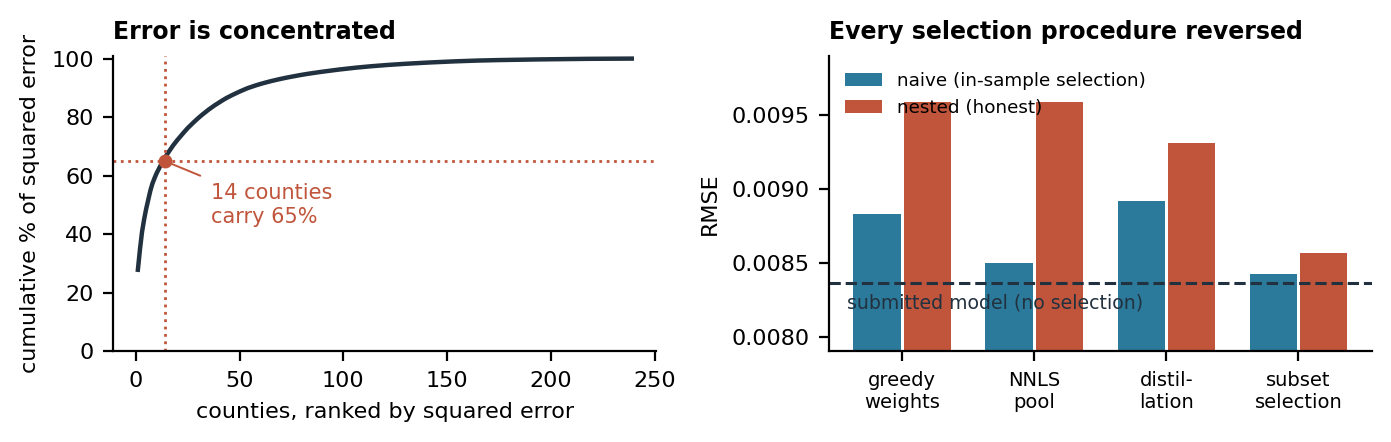
\includegraphics[width=\textwidth]{fig1_concentration_staircase.png}
\caption{\textbf{Left:} squared error is carried by a handful of counties, so
fold composition dominates fold-to-fold variance --- the reason we pair by county
when testing significance. \textbf{Right:} four selection procedures, each
measured naively (choosing on the data it is then scored on) and nested
(choosing on four folds, scoring on the fifth). Bars are within-technique pairs.
Every one reverses; the submitted model performs no selection at all.}
\label{fig:conc}
\end{figure*}

\section{Diagnosis: the error budget}
\label{sec:diag}

Before fitting anything further we decomposed the residual of a trained model
into three interpretable components, using oracle substitutions on cached
out-of-fold predictions. Given a predicted trajectory, we ask how much squared
error would be removed by knowing the true county-level \emph{scale}; by knowing
the true normalised \emph{shape}; and by knowing the optimal per-county temporal
\emph{shift}.

\begin{center}\small
\begin{tabular}{lc}
\toprule
oracle & share of MSE removed \\
\midrule
county scale (magnitude) & $\approx45\%$ \\
trajectory shape & $\approx37\%$ \\
timing ($\pm12$\,h shift) & $16.8\%$ \\
\bottomrule
\end{tabular}
\end{center}

Two consequences follow, and both proved predictive.

\textbf{(i) There is no dominant failure mode.} The budget is spread across three
comparable components. A better \emph{architecture} attacks shape, which is at
most $37\%$ of the problem and only partially recoverable; no architecture can
address scale, which is a property of the county rather than of the sequence.
The diagnosis therefore predicts that architecture substitution should yield
little --- and Section~\ref{sec:ledger} shows nine modern architectures landing
at or behind a plain GRU.

\textbf{(ii) The recoverable part of scale is not the part a model can fix.}
County magnitude is in fact substantially predictable: an out-of-fold
county-holdout model reaches $R^2 = 0.55$--$0.60$, and our shipped model's own
predicted-versus-true county mass has $R^2 = 0.69$ (log) and $0.88$ (raw). What
is \emph{not} recoverable is the \textbf{residual} multiplier once the model has
spoken: regressing $\log(\text{true mass}/\text{predicted mass})$ on every legal
feature gives out-of-fold $R^2 \approx 0$. Since every per-county correction
scheme necessarily targets that residual, the diagnosis predicts they must all
fail. Six independent attempts did.

This distinction matters, and we state it carefully because we previously stated
it too broadly (§\ref{sec:wrong}).

\paragraph{Where the error is not.} $42\%$ of scored cells are exactly zero, yet
they carry $0.7\%$ of the squared error;
$82\%$ of the squared error is under-prediction of outages that did occur,
two thirds of it in 14 counties. A model that first decides whether a cell is
zero therefore has a ceiling of $0.00003$ even with a perfect classifier;
two measured versions gain nothing under nesting. Splitting \emph{counties} instead, with a
random-forest gate on legal features and the best configuration per group,
is worse by $0.0004$; worse by $0.00003$ even with a perfect gate. The
severe counties \emph{are} identifiable in advance (out-of-fold AUC $0.95$);
how far they will go is not.

\section{Deriving the forecaster}
\label{sec:model}

Nothing in the final model was chosen because it won a bake-off. Each component
is forced by a measurement from §\ref{sec:diag} or from the data itself, and was
then checked against the prediction that measurement implied. This section walks
that chain in the order we actually traversed it; Table~\ref{tab:deriv}
summarises it, and the architecture at the end is the consequence rather than
the starting point.

\paragraph{M1: future weather is known for the whole window, and the horizon
(143\,h) is twice the context (72\,h).} This is not time-series extrapolation.
The forcing that causes outages is \emph{observed} for every hour we must
predict, so the task is to interpolate a response to known weather, not to
continue a series. \textbf{Consequence:} an encoder--decoder whose decoder is
driven by known-future covariates, which is the backbone of every sequence
member. It also explains, before we ran them, why generic long-horizon
forecasters transfer poorly here (§\ref{sec:prior}): they assume context $\ge$
horizon and no known future.

\paragraph{M2: 44\% of scored cells are exactly zero and $p_{99}/\mathrm{median}
\approx 10^3$.} A plain squared-error objective on this distribution is
dominated by a handful of peaks while the zero mass contributes gradient noise.
\textbf{Consequence:} a dual raw$/\sqrt{}$ objective, which keeps peaks in the
loss while stabilising the zeros, and a two-part (``hurdle'') component in the
state-space member that models \emph{whether} a county has an outage separately
from \emph{how large} it is. Both were adopted because the target's shape demanded them,
and both beat their single-scale controls.

\paragraph{M3: only 239 counties exist, i.e.\ 191 training sequences per fold.}
This is the governing constraint of the whole project. It says the sequence
models are \emph{variance}-limited, not information-limited, and it makes three
falsifiable predictions at once: extra input channels should \emph{hurt} them;
variance reduction should pay; and model selection should itself be a major
error source. All three held --- external covariates lost 3/3 against their own
controls while helping trees, seed and snapshot averaging paid on every member
that had un-averaged variance left, and four selection procedures reversed under
nesting (§\ref{sec:proto}). \textbf{Consequences:} statics stay out of the
sequence models (D4), variance reduction is applied deliberately (D2), and the
combination is not fitted at all (D3).

\paragraph{M4: the error budget is 45/37/17 with no dominant mode
(§\ref{sec:diag}).} No architecture can address county scale, and shape is at
most 37\% of the problem. \textbf{Consequence:} we stopped buying architecture.
The prediction was that substitutions would be flat, and nine modern architectures duly landed at or behind a plain GRU. The effort went instead into making the members fail differently --- which is where the remaining headroom had to be,
by elimination.

\paragraph{M5: what the model still gets wrong about a county's magnitude is
unpredictable.} Regressing the ratio of true to predicted county mass on every
legal feature gives out-of-fold $R^2 \approx 0$. \textbf{Consequence:} the model contains no calibration
layer, no per-county experts, no severity gate and no retrieval step. Six
independent attempts to add one failed, exactly as predicted.

\paragraph{M6: given M3--M5, the only lever left is making the models fail
differently.}
This is the step that actually produces the ensemble. If scale is unrecoverable,
architecture is flat, and members cannot be improved by feeding them more, then
what is left is to make members \emph{fail differently} and average them.
\textbf{Consequence:} members are constructed to differ along exactly one axis
each --- objective, augmentation, or function class --- and are then selected on
decorrelation rather than on score (D1). This is why the ensemble contains a
stock-flow state-space model that is barely better than decayed persistence, and
why it contains a patch transformer that is mediocre alone.

\paragraph{M7: diversity and quality are coupled, with a sign.} Measuring error
correlation as we varied training procedure showed it rising monotonically with
every variance-reduction step. \textbf{Consequence:} two rules that a pure
search would never surface --- do not apply the blend partner's own technique to
the other members (D2), and remove the member that is simultaneously redundant
and mediocre (D5). For the second, choosing the member to drop on four folds
and applying it to the fifth gave exactly the same score as choosing it on all
five --- no inflation from having chosen.

\paragraph{M8: only 12 training counties have any outage mass after hour 168.}
\textbf{Consequence:} the single quiet-tail scalar, the lone fitted quantity in
the model, nested and worth $0.00002$.

\begin{table}[t]\small\centering
\begin{tabular}{@{}p{2.35cm}p{2.55cm}p{2.35cm}@{}}
\toprule
measurement & forces & confirmed by \\
\midrule
known future, $H>L$ & encoder--decoder on known covariates & Chronos-2 worse than zeros \\
44\% zeros, heavy tail & dual raw$/\sqrt{}$ loss, hurdle & beats single-scale controls \\
191 sequences/fold & no extra inputs; variance reduction; no fitted weights & 3/3 losses; seeds pay; 4 reversals \\
45/37/17 budget & stop buying architecture & 5/5 at or behind GRU \\
residual $R^2\!\approx\!0$ & no calibration layer & 0/12 corrections \\
diversity is the last lever & members differ on one axis; select on decorrelation & worst member is irreplaceable \\
diversity--quality coupling & don't share the partner's technique; drop the redundant member & $P{=}0.011$; zero optimism gap \\
12 tail counties & one nested scalar & $-0.00002$ \\
\bottomrule
\end{tabular}
\caption{The derivation. Every row is a measurement we made before the design
choice it forced, and the experiment that later tested it.}
\label{tab:deriv}
\end{table}

\subsection{The resulting model}

What falls out is an equal-weight blend of two objects,
\[
\hat{y} \;=\; \tfrac{1}{2}\,\mathcal{C}\big[f_1,\dots,f_{11}\big] \;+\; \tfrac{1}{2}\,A,
\]
followed by the quiet-tail correction of M8, where $\mathcal{C}$ combines the
eleven members by \emph{amplitude and shape separately}: the mean of their
county totals times the mean of their normalised trajectories (D5). It has no
fitted parameter and equals the plain mean whenever the members agree on
timing. The blend partner $A$ carries half
the weight alone because it is as good as the whole bracket, and a $1/9$ seat
cannot express that (§\ref{sec:wrong}).

\begin{center}\small
\begin{tabular}{llc}
\toprule
& differs from the others by & RMSE \\
\midrule
$A$ & schedule diversity (25 seeds $\times$ 4 snapshots) & 0.00862 \\
\midrule
\texttt{s51} & dual raw/$\sqrt{}$ loss + snapshots & 0.00884 \\
\texttt{s62} & scoring-aligned hour weights & 0.00897 \\
\texttt{i11} & storm jitter + scoring-aligned weights & 0.00909 \\
\texttt{s35} & mixup augmentation & 0.00912 \\
\texttt{f2} & function class: boosted trees + statics & 0.00930 \\
\texttt{s39} & cross-county attention & 0.00939 \\
\texttt{ts2} & function class: patch transformer & 0.00952 \\
\texttt{s35w} & mixup + scoring-aligned weights & 0.00930 \\
\texttt{r6} & stock-flow + two nested flow scalars & 0.01090 \\
\texttt{p1c} & stock-flow, no rollout training & 0.01148 \\
\texttt{p1b} & function class: stock-flow state space & 0.01042 \\
\bottomrule
\end{tabular}
\end{center}

\noindent \texttt{f2} is the only member consuming data outside the competition
package: terrain, land cover, forest inventory and utility infrastructure, plus
physically motivated interactions (gust\,$\times$\,soil moisture,
canopy\,$\times$\,gust). All are static, public and outage-free, and are bundled
with the code so it runs offline. By M3 they are deliberately withheld from the
sequence members. Should the organisers read the rules as excluding external
data entirely, substituting a package-only variant of \texttt{f2} costs
$0.00004$ --- measured, and shipped as a one-line fallback.

\subsection{The four consequences that were not obvious}

M1--M5 are, in hindsight, forced. Four consequences were not, and each is
carried by a measurement we would not have made without the chain above.

\paragraph{D1 (from M6) --- the worst member is the one to keep.} \texttt{p1b}
is the weakest member by a wide margin --- barely better than decayed
persistence --- and is nonetheless irreplaceable: tested against 27 alternatives
for its seat, \emph{keeping it ranks first of 28}. It is the most decorrelated
model in the set (mean error correlation $0.76$), and that diversity is worth
more than the $0.001$ of solo RMSE it concedes (Fig.~\ref{fig:div}). The same
logic admitted PatchTST, mediocre alone but the second-most decorrelated object
we have.

\paragraph{D2 (from M7) --- improving a member can cost more than it buys.} We can
put a sign on the trade. Applying snapshot ensembling to \texttt{i11} improved
it from $0.00955$ to $0.00892$ --- the best that member ever scored --- and made
the \emph{ensemble significantly worse} ($P{=}0.011$, CI excluding zero),
because the same technique drove its error basis onto $A$'s ($A$ is itself a
snapshot ensemble). Variance reduction buys solo accuracy by \emph{spending}
error diversity; when the partner shares the technique, the exchange rate
eventually turns negative. Re-running all ten remaining members at 25 seeds
each made the point across the set: six improved \emph{alone}, none was
adopted as a swap, and all ten together scored $0.00848$ against $0.00836$.

\begin{figure}[t]
\centering
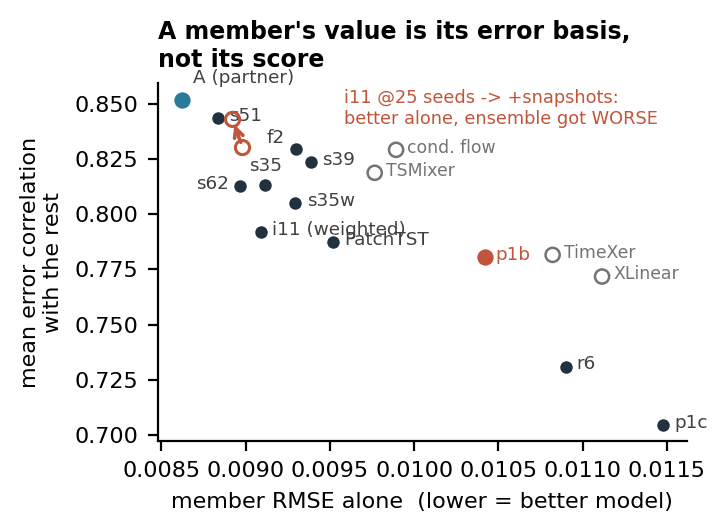
\includegraphics[width=\linewidth]{fig3_diversity.png}
\caption{Every member of the ensemble, positioned by how good it is alone
(horizontal) against how much its errors resemble the rest (vertical). The
useful direction is \emph{down}, not left. The three stock-flow models are the
worst in the set and the only ones far from the crowd, which is why they
survive every replacement test. The arrow shows \texttt{i11} being genuinely improved: it
moves left (better) but also up (more redundant), and the ensemble got worse.}
\label{fig:div}
\end{figure}

\paragraph{D3 (from M3) --- fitting the combination is negative-value.} Every
weight above --- the $1/11$s and the $1/2$ --- is fixed in advance, not tuned. This is measured: fitting the full weight simplex over the three objects buys
$0.000007$, while every selection procedure we tried reversed under nesting
(§\ref{sec:proto}). Exactly two fitted scalars survive, both nested: the
quiet-tail factor, and a rescale on the tabular member, which fits on
$\sqrt{\mathrm{OSI}}$ and squares back and so by Jensen sits $16\%$ below the
conditional mean. Removing that bias \emph{fully} improves that member alone
and makes the ensemble \emph{worse}; the partial rescale all five folds adopt
leaves it shrunk --- shrinkage again, from a third direction.

\paragraph{D4 (from M7) --- one member is dead weight, and it is provable.} A drop-one search over the bracket selects the multi-origin
member on \emph{all five folds}; naive and nested estimates are consequently
\emph{identical}, a zero optimism gap. That member is
simultaneously highly correlated with the rest and mediocre alone --- neither
property alone identifies dead weight.


\paragraph{D5 --- the combination rule is a lever of its own.} Members that
agree on a storm's size but not its hour average into a flatter peak than any
of them predicts: the plain mean spends amplitude to hedge timing. Averaging
each member's county total and its normalised shape separately keeps the
amplitude, with no fitted parameter. Under that rule a nested add-one sweep
over every cached object admitted three more members on every fold --- two
further stock-flow variants and the weighted mixup model; doubling the
existing physics member's weight does not help, so these are new bases. Choosing among all ten
configurations searched on four folds and applying the choice to the fifth
gives 0.00838, against 0.00847 for the eight-member mean. It leaves the
dominant error untouched: the under-prediction share moves from $81.9\%$ to
$81.6\%$.

\subsection{Coverage of the search}

The search was organised by family rather than by inspiration. Table~\ref{tab:cov}
summarises 156 ranked experiments; roughly 20 further ablations and audits are
not scored here.

\begin{table}[ht]\small\centering
\begin{tabular}{lcc}
\toprule
family & runs & best RMSE \\
\midrule
tabular / feature engineering & 31 & 0.00938 \\
sequence architectures & 24 & 0.00897 \\
augmentation & 11 & 0.00893 \\
feature \& member selection & 10 & 0.00934 \\
variance reduction & 16 & 0.00863 \\
neural-tabular (MLP, KAN, TabNet, FT-T) & 5 & 0.00989 \\
stock-flow / physical & 8 & 0.01025 \\
diversity-directed training & 4 & 0.00920 \\
multi-stage (hurdle, two/three-stage) & 6 & 0.00945 \\
hyperparameter tuning (Ray, Optuna) & 4 & 0.00914 \\
objective / loss design & 10 & 0.00888 \\
attention / graph & 3 & 0.00931 \\
kernel, linear, decomposition & 6 & 0.01017 \\
generative / pretrained (flow, Chronos-2) & 3 & 0.00989 \\
other (calibration, retrieval, adaptation) & 15 & 0.00904 \\
\bottomrule
\end{tabular}
\caption{Experiment coverage. Every row uses the identical protocol of
§\ref{sec:proto}, so all entries are directly comparable.}
\label{tab:cov}
\end{table}

\section{Predicted versus measured}
\label{sec:ledger}

If the diagnosis in §\ref{sec:diag} is real, it should have predicted our
experimental record \emph{including the failures}. It does. Each row below is a
prediction of the diagnosis and the experiments that tested it.

\begin{center}\small
\begin{tabular}{p{3.4cm}p{3.4cm}c}
\toprule
prediction & experiments & \\
\midrule
Post-model residual is unrecoverable $\Rightarrow$ per-county corrections fail &
residual calibration; severity-gated experts; restoration rates; analog
retrieval; external county data; test-time latent adaptation & 0/6 \\
\addlinespace
Scale comes from \emph{static} attributes, not the prefix & static enrichment of
the tabular member & \checkmark \\
\addlinespace
No dominant failure mode $\Rightarrow$ architecture cannot unlock a step change &
TCN, N-BEATS, TiDE, TFT-lite, multi-task & 0/5 \\
\addlinespace
Sequence models are variance- not information-limited & extra input channels hurt
them while the \emph{same} inputs help trees & 3/3 \\
\addlinespace
Variance reduction and diversity must pay & seed averaging, snapshot ensembling,
augmentation, ensembling & \checkmark \\
\bottomrule
\end{tabular}
\end{center}

The six failed residual attacks are worth one line each because their failure is
the evidence: per-county residual calibration degraded RMSE from $0.00937$ to
$0.01099$; severity-gated experts scored $0.01106$ with predicted gates versus
$0.00966$ with oracle gates, so the entire gap is gate error; per-county
restoration rates $0.01131$; retrieval of analog futures $0.01045$; external
county data in a sequence model $0.00956$ against its own $0.00910$ control; and
test-time latent adaptation changed the score in the eighth decimal against an
identical-architecture control.

Roughly 45 negative results therefore act as a validation set for the
diagnosis.

\begin{figure*}[t]
\centering
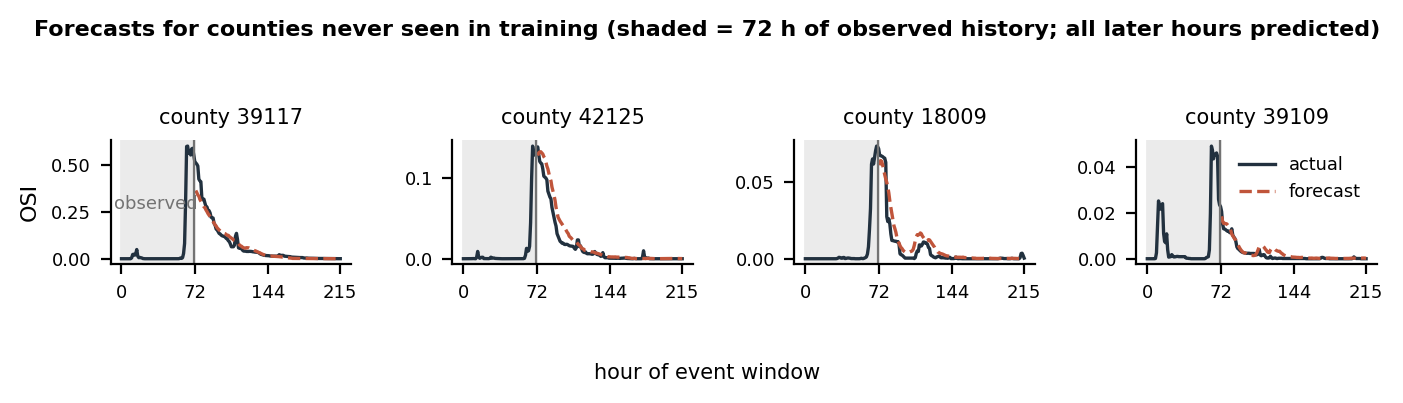
\includegraphics[width=\textwidth]{fig2_trajectories.png}
\caption{Out-of-fold forecasts for four held-out counties spanning an order of
magnitude in severity. The model sees only the shaded 72 hours of outage history
for these counties --- every later hour is predicted --- yet reproduces onset
timing, peak magnitude and the multi-day restoration decay, including the
second wave visible in the right-hand panel.}
\label{fig:traj}
\end{figure*}

\section{Results and critical discussion}
\label{sec:results}

\begin{center}\small
\begin{tabular}{lcc}
\toprule
model & RMSE & MAE \\
\midrule
all-zeros & 0.01632 & 0.00399 \\
decayed persistence & 0.01110 & 0.00307 \\
best single model ($A$) & 0.00862 & 0.00247 \\
\textbf{submitted ensemble}, nested & \textbf{0.00838} & \textbf{0.00255} \\
\bottomrule
\end{tabular}
\end{center}
Figure~\ref{fig:traj} shows the resulting forecasts.
The ensemble improves on the strongest naive baseline by $25\%$ and on all-zeros
by $49\%$, both significant under a paired county bootstrap.

\textbf{Uncertainty.} Split-conformal $90\%$ intervals, calibrated on four
folds and checked on the fifth, cover $0.900$ of held-out cells at every
horizon; scaling the residual by the prediction narrows them by $22$--$48\%$
at the same coverage; the point forecast is unchanged.

\textbf{We do not claim the differences among our own top models are
significant.} They are not. Resampling the 63 scored counties
gives a score standard deviation of \textbf{0.0016} --- roughly $45\times$ the
margin separating our final model from our own earlier ones, and larger than the
entire spread of the 2025 finalist field. Any ranking among comparable
submissions on this task is substantially a statement about which counties
happened to be held out.

\textbf{Where the remaining error lives.} It is concentrated: 14 counties carry
two-thirds of it, and it is dominated by county scale, which our own
diagnosis says is only partially recoverable and whose residual is not
recoverable at all from the data provided. We believe the practical ceiling on
this task, given 72 hours of history for counties never observed, is not far
below where we are --- and that closing it requires different \emph{data}
(sub-county asset and vegetation exposure, crew allocation), not a different
model.

\textbf{Operational reading.} For a utility, the useful output is not the point
forecast but the concentration: the model reproduces the observed
predicted-versus-true county mass relationship with $R^2 = 0.88$, which is what
supports crew pre-positioning, while the per-county residual multiplier it cannot
predict is the quantity that would justify reallocating crews mid-event. The
two quantities are separable, and the model delivers only the first.

\section{What we got wrong}
\label{sec:wrong}

An audit of our own measurements found four defects. Each is given below with
what it changed.

\textbf{1. A circular shift inflated a headline claim.} Our timing oracle used a
wrapped array shift, which folded the quiet tail into the storm onset and
penalised every nonzero offset. We had concluded that ``phase is essentially
free'' at $2\%$ of MSE. With a physically correct edge-padded shift the true
figure is \textbf{16.8\%}. A claim we had planned to lead with was withdrawn, and
a rejected experiment was reopened.

\textbf{2. An over-broad law.} We had claimed county magnitude was
``not identifiable from the prefix, $R^2 \le 0.08$''. That came from one
in-sample construction against a fixed sub-window. Re-derived four ways, magnitude
is substantially predictable ($R^2$ up to $0.88$); only the post-model residual is
not. The experimental verdicts are unchanged --- all six attacks targeted the
residual --- but the stated law was wrong.

\textbf{3. A metric mismatch.} Our significance-testing script pooled squared
error across horizons, while every headline number was the mean of four
per-horizon RMSEs. We corrected it and re-ran every adoption comparison; no
adoption or rejection verdict changed.

\textbf{4. A saturation finding that was a statement about the test.} Twelve
consecutive experiments indicated the ensemble was saturated. The test used a
$1/9$ weight seat, which arithmetically caps any added object's effect in the
fifth decimal regardless of quality. Giving an equally good model a full half
weight instead improved the model by $0.00008$ --- the second-largest single gain
in the project.

Defects 1 and 4 share a cause worth naming: a \emph{convenient} construction
standing in for a faithful one. Both surfaced by re-deriving a number rather
than by running a new model.

\section{Relation to prior work}
\label{sec:prior}

Two literatures touch this problem and neither addresses its shape. Operational
outage modelling predicts storm \emph{totals} or damage counts from forecast
weather, typically with tree ensembles or GLMs on static exposure; it does not
produce hourly trajectories. The EAGLE-I-era nowcasting work produces hourly
outage forecasts but at 1--6\,h horizons with the target's own recent history
available. Our task is neither: a 144-hour horizon, for counties whose history is
withheld, with future weather fully known. We found no published treatment of
that combination. The nearest general tools are the recent long-horizon
architectures built for exogenous drivers --- TimeXer~\cite{timexer},
XLinear~\cite{xlinear}, TSMixer~\cite{tsmixer} --- and the pretrained
forecasters that now accept covariates, Chronos-2~\cite{chronos2} among them.
We ran each on our protocol. Zero-shot Chronos-2 given our 23 weather
covariates scores 0.0214, worse than predicting zero everywhere (0.0163), and
the covariates make it slightly worse than without them (0.0201): it predicts a
non-zero level almost everywhere, where 42\% of the truth is exactly zero. The
three architectures, adapted to read the future weather, score
0.0098--0.0111 alone
and each makes the blend worse when added as a ninth member; nested selection
keeps none. A conditional normalizing flow trained by likelihood, with the
sample mean as its point forecast, scores 0.0099 and is not admitted either.

The element we did not find in prior work is the \emph{use} of an error budget
as a filter applied \emph{before} the experiments. Oracle decompositions are
not new, and neither is
nested validation. What we have not seen is a forecasting study that computes
the decomposition first, derives from it which \emph{classes} of intervention can
pay, and then reports the full experimental ledger --- negative results
included --- as a test of that derivation. Section~\ref{sec:ledger} is that
test.

\section{Conclusion}

The strongest claim we can defend is not the score but the method that produced
it: measure the error budget first, use it to rule families of interventions in
or out, validate at the unit you will be evaluated on, and nest anything learned
across folds. That discipline cost four apparent wins worth up to $0.0008$
apiece, each of which we would otherwise have reported. Resampling the 63 scored
counties moves the score by $0.0016$, so we make no claim to separation from
comparable submissions at the fifth decimal.

\section{Reproducibility}

The submitted code runs end-to-end on the provided data files with fixed seeds.
A clean-clone drill --- a fresh export of the repository with only the three
competition CSVs restored --- reproduces the submitted prediction file with a
\textbf{byte-identical SHA-256}. A standalone verifier re-derives every format
expectation from the template and the competition calendar rather than trusting
the writer that produced the file; it checks row count, column order, identifier
byte-identity, the exact NaN pattern implied by the horizon calendar, and that
all predictions lie in $[0,1]$. All headline figures in this report are
regenerated from cached out-of-fold predictions by a single script, so any number
here can be checked by re-running it rather than by trusting us.

{\footnotesize
\begin{thebibliography}{9}\small
\bibitem{zeng} A.~Zeng et al. Are transformers effective for time series
forecasting? \emph{AAAI}, 2023.
\bibitem{nie} Y.~Nie et al. A time series is worth 64 words: long-term
forecasting with transformers. \emph{ICLR}, 2023.
\bibitem{liu} Y.~Liu et al. iTransformer: inverted transformers are effective
for time series forecasting. \emph{ICLR}, 2024.
\bibitem{tan} M.~Tan et al. Are language models actually useful for time series
forecasting? \emph{NeurIPS}, 2024.
\bibitem{huang} G.~Huang et al. Snapshot ensembles: train 1, get M for free.
\emph{ICLR}, 2017.
\bibitem{zhang} H.~Zhang et al. mixup: beyond empirical risk minimization.
\emph{ICLR}, 2018.
\bibitem{cawley} G.~Cawley and N.~Talbot. On over-fitting in model selection and
subsequent selection bias in performance evaluation. \emph{JMLR}, 11:2079--2107,
2010.
\bibitem{kim} T.~Kim et al. Reversible instance normalization for accurate
time-series forecasting against distribution shift. \emph{ICLR}, 2022.
\bibitem{timexer} Y.~Wang et al. TimeXer. \emph{NeurIPS}, 2024.
\bibitem{xlinear} Z.~Ma et al. XLinear. arXiv:2601.09237, 2026.
\bibitem{tsmixer} S.-A. Chen et al. TSMixer. \emph{TMLR}, 2023.
\bibitem{chronos2} A.~F. Ansari et al. Chronos-2. arXiv:2510.15821, 2025.
\end{thebibliography}}

\end{document}
